\section{User Stories compatible Angular - Twig}
	\paragraph{}
		Seul l'aspect graphique changera entre la version Twig et la version Angular.
		Pour plus de détails rendez-vous au chapitre \ref{chap:Séparation backend frontend}
	
	\subsection{En tant qu’utilisateur, je dois pouvoir me connecter sur le site}
		\subsubsection{Différences}
	\begin{itemize}
		\item Réalisation d'une requête POST via l'api REST permettant d'effectuer l'authentification dans le backend. 
		\item Différences au niveau de l'aspect graphique de la page de connection. 
		\item Connection via l'adresse Email et non le nom d'utilisateur. 
		\item Redirection automatique de l'utilisateur vers la page de connection lors de l'accès au site si l'utilisateur n'est pas connecté.
		\item Utilisation d'un LoginAuthenticator afin de pouvoir authentifier l'utilisateur dans le backend. 
		\item Utilisation de coockies pour préserver les informations de l'utilisateur. 
	\end{itemize}

\newpage
\subsubsection{Diagramme de séquence}
	\begin{figure*}[h!]
		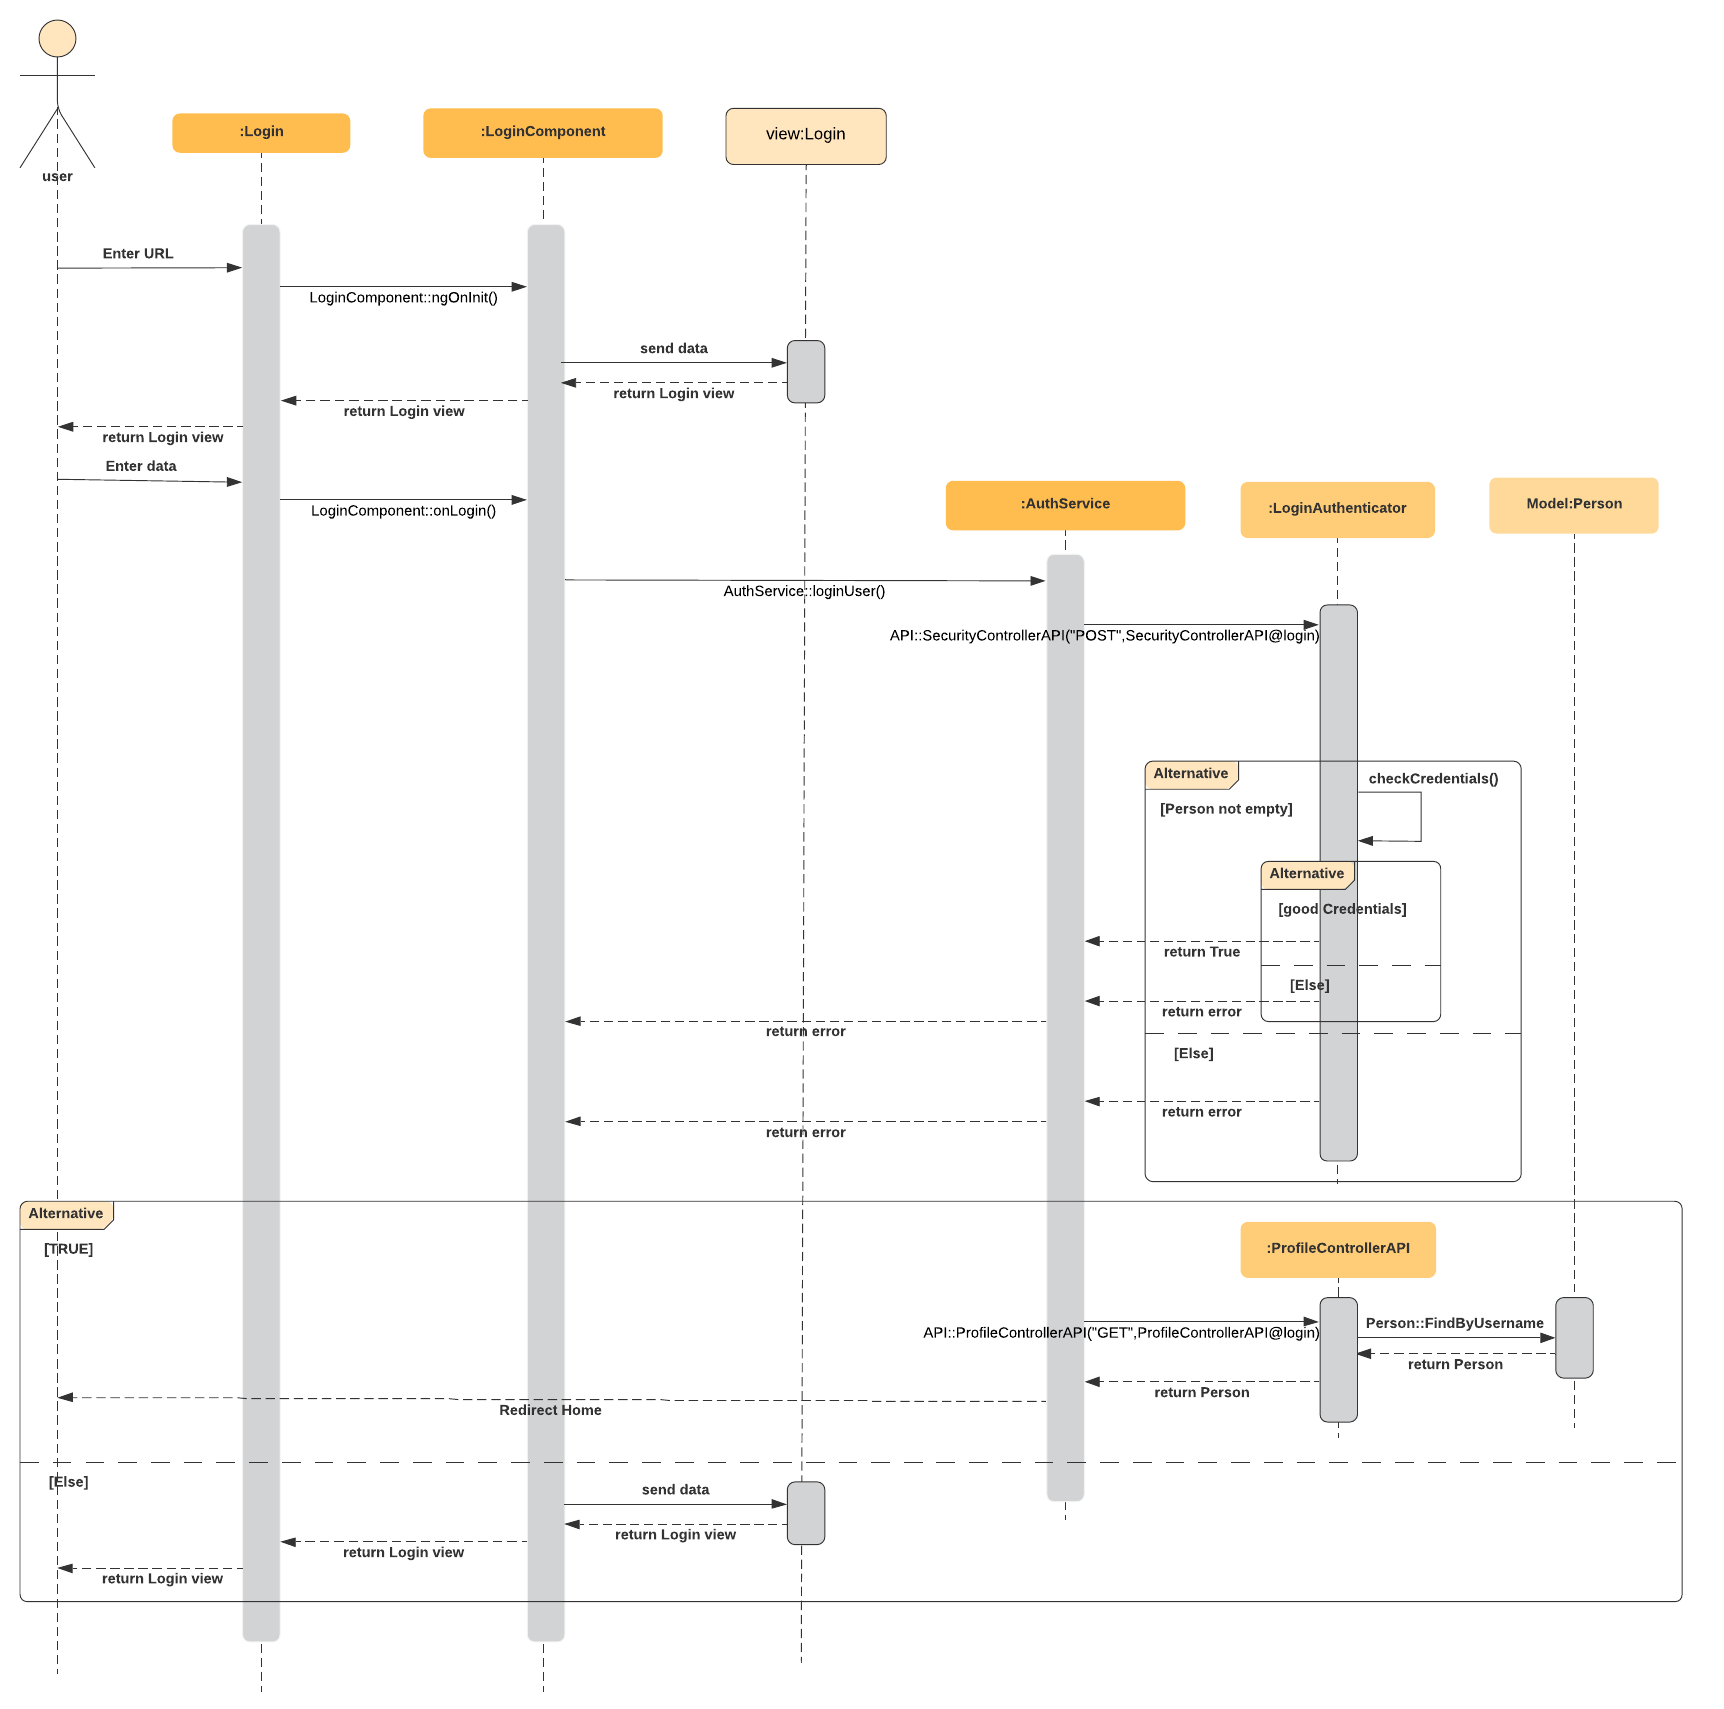
\includegraphics[width =\textwidth,center]{Diagramme/sequence-us0-angular}
		\caption{Diagramme de séquence de la connection d'un utilisateur}
	\end{figure*}

\newpage
\subsubsection{Scripts concernés}
	\begin{itemize}
		\item \Href{https://github.com/victorsmits/Aquabike/blob/master/frontend/src/app/service/api.service.ts}{api.service.ts}
		\item \Href{https://github.com/victorsmits/Aquabike/blob/master/frontend/src/app/service/auth.service.ts}{auth.service.ts}
		\item \Href{https://github.com/victorsmits/Aquabike/blob/master/backend/src/Controller/API/SecurityControllerAPI.php}{SecurityControllerAPI.php}
		\item \Href{https://github.com/victorsmits/Aquabike/blob/master/backend/src/Controller/API/ProfileControllerAPI.php}{ProfileControllerAPI.php}
		\item \Href{https://github.com/victorsmits/Aquabike/blob/master/frontend/src/app/login/login.component.ts}{login.component.ts}
		\item \Href{https://github.com/victorsmits/Aquabike/blob/master/frontend/src/app/login/login.component.html}{login.component.html}
		\item \Href{https://github.com/victorsmits/Aquabike/blob/master/backend/src/Entity/Person.php}{Person.php}
	\end{itemize}
	
	\vspace{\baselineskip}
	\subsection{En tant qu’utilisateur, je dois pouvoir me créer un compte sur le site}
		\begin{figure}[h]
	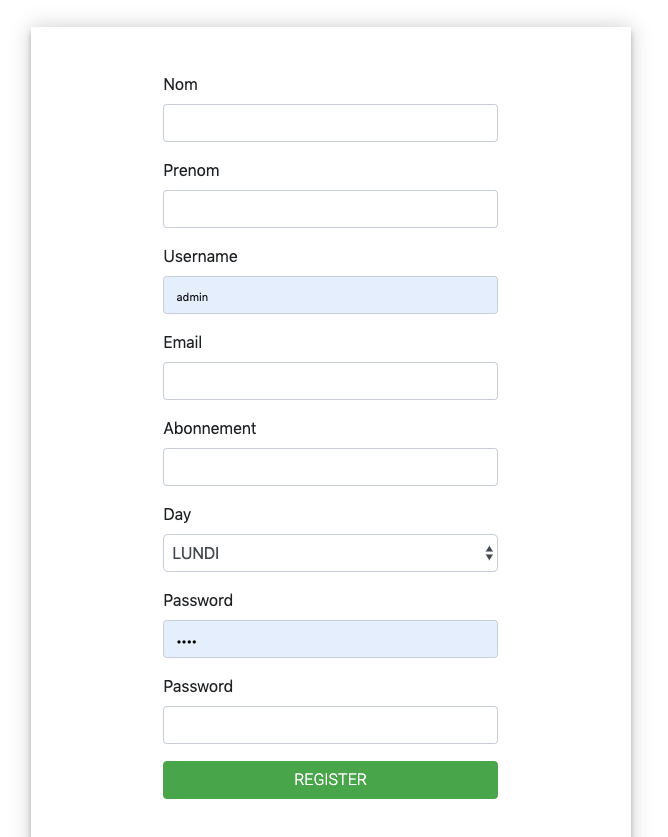
\includegraphics[width=0.5\textwidth,center]{Figures/us1-1}
	\caption{Formulaire d'inscription}
\end{figure}

\vspace{\baselineskip}
\begin{enumerate}
	\item L'utilisateur rentre ses information dans le formulaire. 
	\item L'utilisateur sélectionne le type de session à laquelle il est inscrit. 
	\item L'utilisateur clique sur \textit{Register} et attend la redirection. 
\end{enumerate}

\newpage
\subsubsection{Gestion des erreurs et sécurité}
	\paragraph{}
		\begin{itemize}
			\item L'utilisateur doit remplir tous les champs. Si un champ est manquant, une erreur apparaitra. 
			\item Le nom d'utilisateur et l'adresse Email sont uniques dans le système, s'il entre un Email ou nom d'utilisateur déjà existant, une erreur lui dira de corriger.
			\item L'utilisateur doit confirmer son mot de passe, si les mots de passe sont différents ou plus petits que 6 charactères il y aura un message d'erreur.
		\end{itemize}
		
\subsubsection{Diagramme de séquence}
	\begin{figure}[h]
		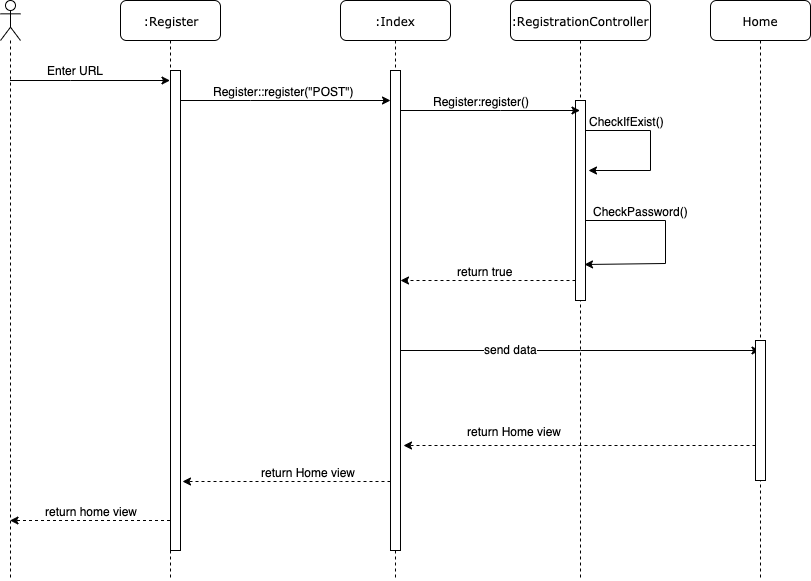
\includegraphics[width=0.8\textwidth,center]{Diagramme/sequence-us1}
		\caption{Diagramme de séquence de l'enregistrement d'un nouvelle utilisateur. }
	\end{figure}
	
	
\subsubsection{Scripts concernés}
	\begin{itemize}
		\item \Href{https://github.com/victorsmits/Aquabike/blob/master/backend/src/Controller/RegistrationController.php}{RegistrationController.php}
		\item \Href{https://github.com/victorsmits/Aquabike/blob/master/backend/templates/registration/register.html.twig}{register.html.twig}
		\item \Href{https://github.com/victorsmits/Aquabike/blob/master/backend/src/Entity/Person.php}{Person.php}
	\end{itemize}

	\vspace{\baselineskip}
	\subsection{En tant qu'utilisateur, je dois pouvoir sélectionner le mois et l'année pour afficher les sessions qui m'intéressent}
		\begin{figure*}[h]
	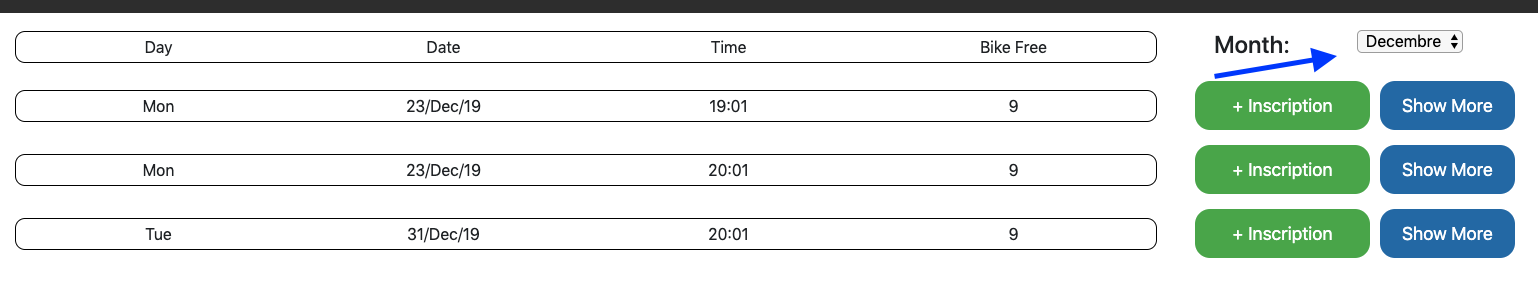
\includegraphics[width = 0.8\textwidth,center]{Figures/us2-1}
	\caption{selection du mois et de l'année}
\end{figure*}

\begin{enumerate}
	\item L'utilisateur choisit le mois et l'année. 
	\item la liste se rafraîchis afin de correspondre à la selection
\end{enumerate}
	
	\newpage
	\subsection{En tant qu’utilisateur, je dois pouvoir m’inscrire à une session un certain jour}
		\begin{figure*}[!h]
	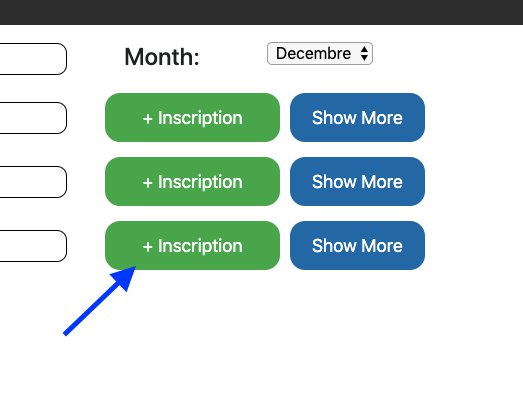
\includegraphics[width=0.5\textwidth,center]{Figures/us3-1}
	\caption{bouton d'inscritption}
\end{figure*}

\begin{enumerate}
	\item l'utilisateur choisit la session correspondant à sa demande.
	\item l'utilisateur clique sur le bouton  \textit{+ Inscription}
\end{enumerate}

\subsubsection{Gestion des erreurs}
	\begin{itemize}
		\item Si l'utilisateur ne possède plus d'abonnement, une erreur sera affichée lui signalant le problème. 
		\item Si la session est complète un message d'erreur sera affiché. 
	\end{itemize}
	
\subsubsection{Scripts concerné}
	\begin{itemize}
		\item \Href{https://github.com/victorsmits/Aquabike/blob/master/Symfony-Twig/src/Controller/MonthController.php}{MonthController.php}
		\item \Href{https://github.com/victorsmits/Aquabike/blob/master/Symfony-Twig/templates/month/month.html.twig}{month.html.twig}
		\item \Href{https://github.com/victorsmits/Aquabike/blob/master/Symfony-Twig/src/Entity/Session.php}{Session.php}
	\end{itemize}

	\newpage
	\subsection{En tant qu’utilisateur, je dois pouvoir être inscrit automatiquement à une session}
		\subsubsection{Différences}
	\begin{itemize}
		\item Réalisation de l'inscription automatique au session lors de l'enregistrement de l'utilisateurs. 
		\item Utilisation de type de session afin de facilité et de multiplier le choix des abonnements possible. 
		\item Possibilité pour un utilisateur de s'inscrire à plus de un type de session par semaine. 
		\item Sélection du type de session parmi une liste. 
	\end{itemize}

	\begin{figure*}[h!]
		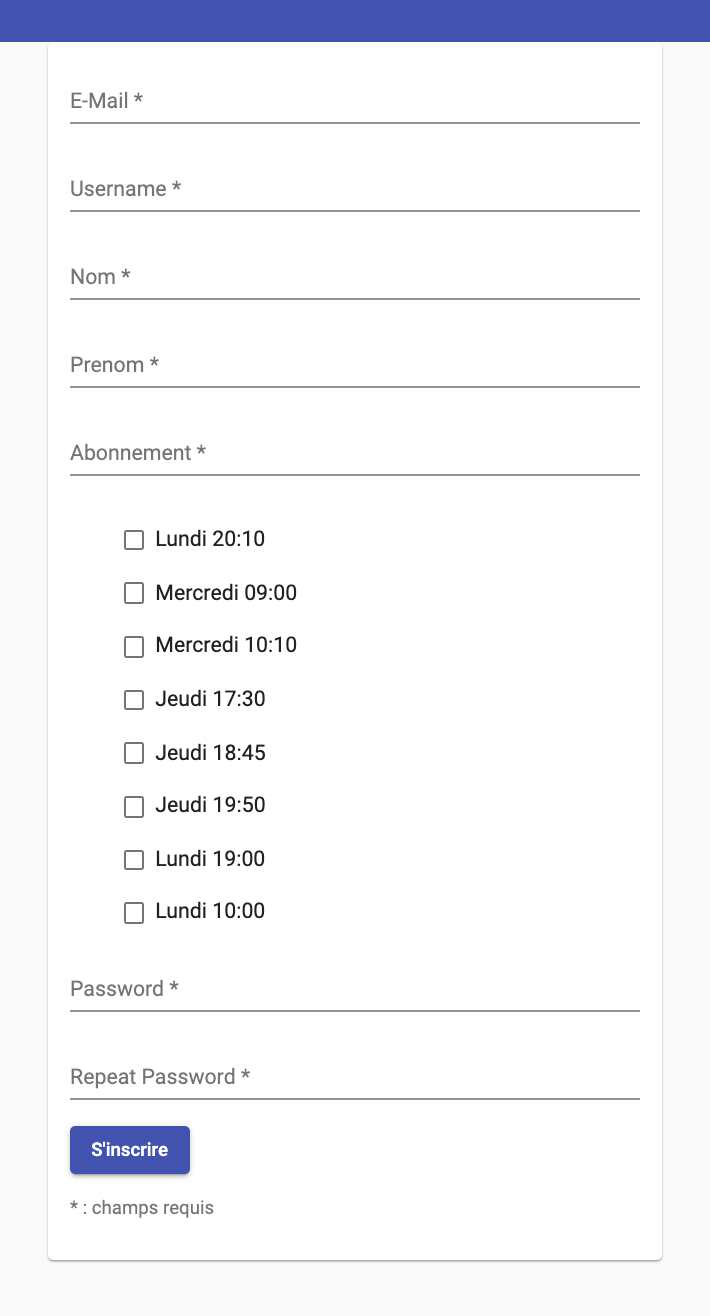
\includegraphics[width = 0.5\textwidth,center]{Figures/us4-1-angular}
		\caption{Formulaire d'inscription version angular}
	\end{figure*}
	
	
\newpage
\subsubsection{Diagramme de séquence}
	\begin{figure}[h]
		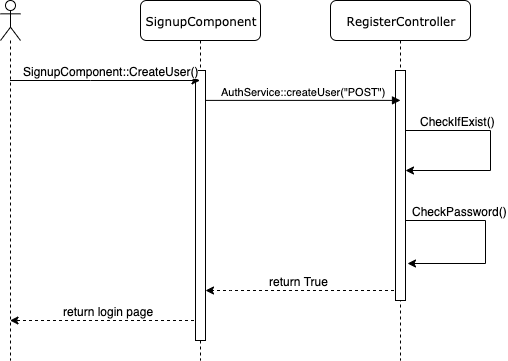
\includegraphics[width=\textwidth,center]{Diagramme/sequence-us1-angular}
		\caption{Diagramme de séquence de l'inscription automatique d'un utilisateur. }
	\end{figure}

\vspace{\baselineskip}
\subsubsection{Script concernés}
	\begin{itemize}
		\item \Href{https://github.com/victorsmits/Aquabike/blob/master/frontend/src/app/service/auth.service.ts}{auth.service.ts}
		\item \Href{https://github.com/victorsmits/Aquabike/blob/master/backend/src/Controller/API/SecurityControllerAPI.php}{SecurityControllerAPI.php}
		\item \Href{https://github.com/victorsmits/Aquabike/blob/master/backend/src/Entity/TypeSession.php}{TypeSession.php}
		\item \Href{https://github.com/victorsmits/Aquabike/blob/master/backend/src/Entity/Session.php}{Session.php}
		\item \Href{https://github.com/victorsmits/Aquabike/blob/master/backend/src/Entity/Inscription.php}{Inscription.php}
		\item \Href{https://github.com/victorsmits/Aquabike/blob/master/backend/src/Entity/Person.php}{Person.php}
		\item \Href{https://github.com/victorsmits/Aquabike/blob/master/frontend/src/app/signup/signup.component.ts}{signup.component.ts}
		\item \Href{https://github.com/victorsmits/Aquabike/blob/master/frontend/src/app/signup/signup.component.html}{signup.component.html}
	\end{itemize}
	
	\vspace{\baselineskip}
	\subsection{En tant qu’utilisateur, je dois pouvoir me désinscrire à une session}
		\begin{figure*}[h]
	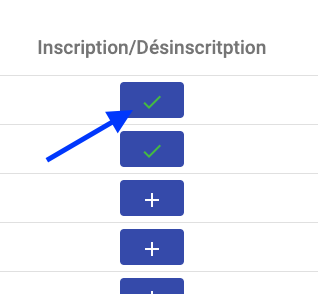
\includegraphics[width=0.5\textwidth,center]{Figures/us5-1}
	\caption{Bouton de désinscription à une session}
\end{figure*}

\begin{enumerate}
	\item L'utilisateur trouve la session qui l'interesse.
	\item Le check vert indique qu'il est inscrit.
	\item Il clique sur le bouton.
\end{enumerate}

\vspace{\baselineskip}
\subsubsection{Script concernés}
	\begin{itemize}
		\item \href{https://github.com/victorsmits/Aquabike/blob/master/backend/src/Controller/MonthController.php}{MonthController.php}
		\item \href{https://github.com/victorsmits/Aquabike/blob/master/backend/templates/registration/month.html.twig}{month.html.twig}
		\item \href{https://github.com/victorsmits/Aquabike/blob/master/backend/src/Entity/Person.php}{Person.php}
		\item \href{https://github.com/victorsmits/Aquabike/blob/master/backend/src/Entity/Inscription.php}{Inscription.php}
	\end{itemize}

	\vspace{\baselineskip}
	\subsection{En tant qu’utilisateur, je dois pouvoir voir qui est inscrit pour chaque session}
		\vspace{\baselineskip}
\begin{figure}[h]
	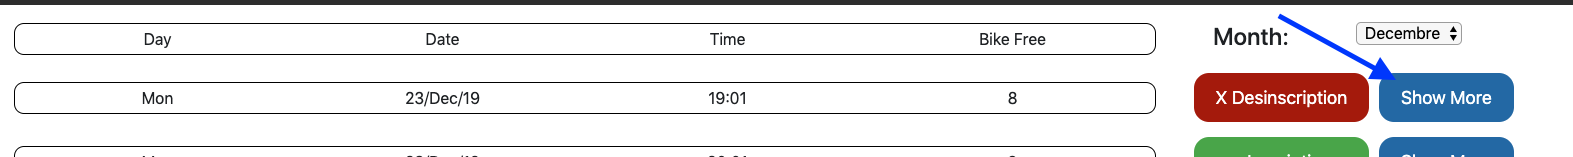
\includegraphics[width=0.9\textwidth,center]{Figures/us6-1}
	\caption{Bouton d'affichage}
\end{figure}

\begin{figure}[h]
	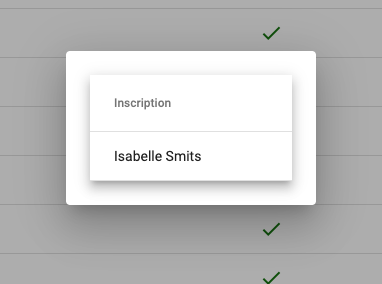
\includegraphics[width=0.5\textwidth,center]{Figures/us6-2}
	\caption{Liste Participant(e)s}
\end{figure}

\begin{enumerate}
	\item L'utilisateur trouve la session qui l'intéresse. 
	\item L'utilisateur clique sur le bouton information dans la colonne \textit{Liste Participant(e)s}. 
	\item Un tableau s'affiche avec la liste des inscrit(e)s. 
\end{enumerate}
	
	\newpage
	\subsection{En tant qu’utilisateur, je veux pouvoir voir le nombre de séances qui restent dans mon abonnement}
		\begin{enumerate}
	\item L'utilisateur clique sur son nom dans la bar de navigation.
	\item L'utilisateur est redirigé vers sa page de profil. 
	\item L'utilisateur retrouve l'information dans le cadre afficher sur la page.
\end{enumerate}

\vspace{\baselineskip}
\begin{figure}[h]
	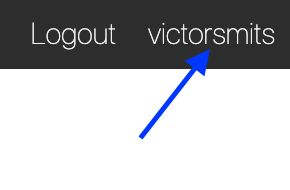
\includegraphics[width=0.5\textwidth,center]{Figures/us7-1}
	\caption{Bouton de navigation vers le profil}
\end{figure}

\vspace{\baselineskip}
\begin{figure}[h]
	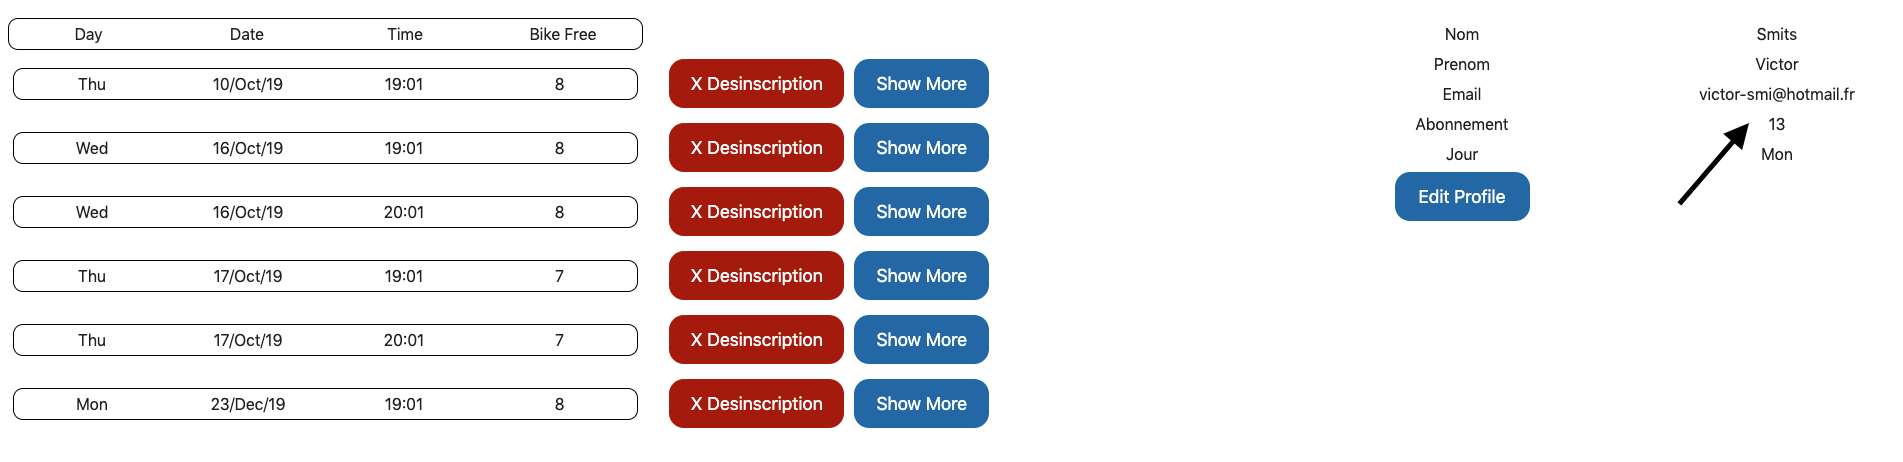
\includegraphics[width=0.9\textwidth,center]{Figures/us7-2}
	\caption{Nombre de séance restante dans l'abonnement}
\end{figure}


\vspace{\baselineskip}
\subsubsection{Script concernés}
	\begin{itemize}
		\item \Href{https://github.com/victorsmits/Aquabike/blob/master/backend/src/Controller/ProfileController.php}{ProfileController.php}
		\item \Href{https://github.com/victorsmits/Aquabike/blob/master/backend/templates/registration/profile.html.twig}{profile.html.twig}
		\item \Href{https://github.com/victorsmits/Aquabike/blob/master/backend/src/Entity/Person.php}{Person.php}
	\end{itemize}


	\vspace{\baselineskip}	
	\subsection{En tant qu'utilisateur, je veux pouvoir modifier mon profil}
		\begin{enumerate}
	\item L'utilisateur clique sur son nom dans la bar de navigation.
	\item L'utilisateur clique sur \textit{Profil} dans le menu déroulant.
	\item L'utilisateur clique sur le bouton edit au dessus de son profil. 
	\item Une fenêtre apparait. 
	\item L'utilisateur rentre les information qu'il souhaite changer. 
	\item L'utilisateur confirm en cliquant sur \textit{ok}
\end{enumerate}

\vspace{\baselineskip}
\begin{figure}[h]
	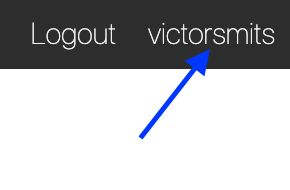
\includegraphics[width=0.4\textwidth,center]{Figures/us7-1}
	\caption{Bouton de navigation vers le profil}
\end{figure}

\begin{figure}[h]
	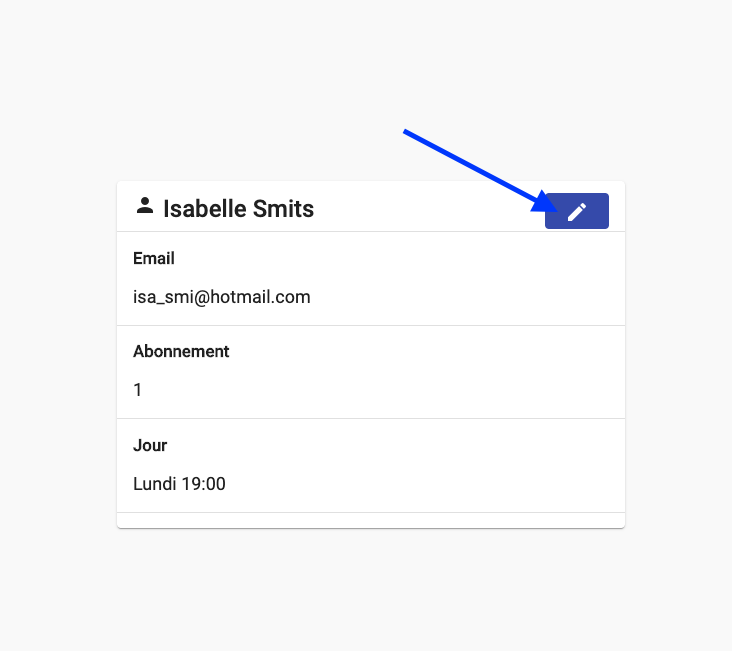
\includegraphics[width=0.4\textwidth,center]{Figures/us8-1}
	\caption{Bouton de modification du profil}
\end{figure}

\newpage
\begin{figure}[h]
	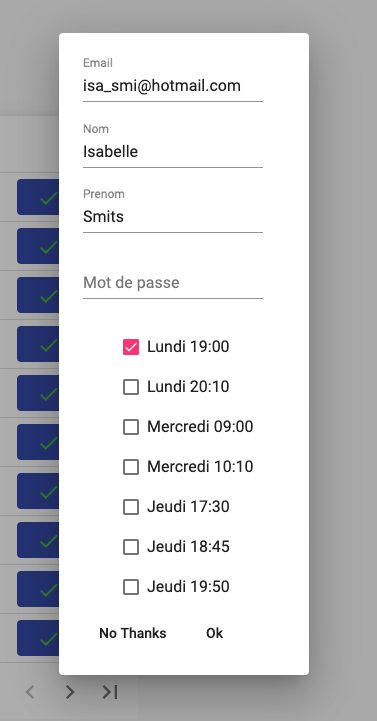
\includegraphics[width=0.4\textwidth,center]{Figures/us8-2}
	\caption{Fenêtre de modification des données du profil}
\end{figure}

	\vspace{\baselineskip}
	\subsection{En tant qu’administrateur, je dois pouvoir annuler une session}
		\subsubsection{Différences}
	\begin{itemize}
		\item Modification graphique du bouton d'annulation de la session. 
	\end{itemize}

\vspace{\baselineskip}
\subsubsection{Scripts concernés}
	\begin{itemize}
		\item \Href{https://github.com/victorsmits/Aquabike/blob/master/frontend/src/app/service/api.service.ts}{api.service.ts}
		\item \Href{https://github.com/victorsmits/Aquabike/blob/master/backend/src/Controller/API/SessionAdministrationControllerApi.php}{SessionAdministrationControllerApi.php}
		\item \Href{https://github.com/victorsmits/Aquabike/blob/master/backend/src/Entity/Session.php}{Session.php}
		\item \Href{https://github.com/victorsmits/Aquabike/blob/master/frontend/src/app/admin-session/admin-session.component.ts}{admin-session.component.ts}
		\item \Href{https://github.com/victorsmits/Aquabike/blob/master/frontend/src/app/admin-session/admin-session.component.html}{admin-session.component.html}
	\end{itemize}

	\newpage
	\subsection{En tant qu'administrateur, je dois pouvoir créer une nouvelle session peu importe la date}
		\subsubsection{Différence}
	\begin{itemize}
		\item Modification graphique du formulaire de création de session. 
	\end{itemize}
	
\vspace{\baselineskip}
\subsubsection{Script concernés}
	\begin{itemize}
		\item \href{https://github.com/victorsmits/Aquabike/blob/master/frontend/src/app/service/api.service.ts}{api.service.ts}
		\item \href{https://github.com/victorsmits/Aquabike/blob/master/backend/src/Controller/API/CreateSessionControllerApi.php}{CreateSessionControllerApi.php}
		\item \href{https://github.com/victorsmits/Aquabike/blob/master/backend/src/Entity/Session.php}{Session.php}
		\item \href{https://github.com/victorsmits/Aquabike/blob/master/frontend/src/app/admin-create-session/admin-create-session.component.ts}{admin-create-session.component.ts}
		\item \href{https://github.com/victorsmits/Aquabike/blob/master/frontend/src/app/admin-create-session/admin-create-session.component.html}{admin-create-session.component.html}
	\end{itemize}

	\newpage
	\subsection{En tant qu'administrateur, je dois pouvoir gérer les abonnement des utilisateurs}
		\subsubsection{Différence}
	\begin{itemize}
		\item Modification graphique de l'affichage des utilisateurs enregistré dans le système. 
	\end{itemize}

\vspace{\baselineskip}
\subsubsection{Script concernés}
	\begin{itemize}
		\item \href{https://github.com/victorsmits/Aquabike/blob/master/frontend/src/app/service/api.service.ts}{api.service.ts}
		\item \href{https://github.com/victorsmits/Aquabike/blob/master/backend/src/Controller/API/AbonnementControllerApi.php}{AbonnementControllerApi.php}
		\item \href{https://github.com/victorsmits/Aquabike/blob/master/backend/src/Entity/Person.php}{Person.php}
		\item \href{https://github.com/victorsmits/Aquabike/blob/master/frontend/src/app/admin-abo/admin-abo.component.ts}{admin-abo.component.ts}
		\item \href{https://github.com/victorsmits/Aquabike/blob/master/frontend/src/app/admin-abo/admin-abo.component.html}{admin-abo.component.html}
	\end{itemize}
